% Build with XeLaTeX (Indic scripts): xelatex main && bibtex main && xelatex main && xelatex main
% Overleaf: Menu > Compiler > XeLaTeX.  acl.sty and acl_natbib.bst are the unmodified official ACL style files.
\PassOptionsToPackage{table}{xcolor}   % row shading in tables (acl.sty loads xcolor)
\documentclass[11pt]{article}

% `preprint' is the official ACL option that shows author names and affiliations (the demo track is single-blind).
\usepackage[preprint]{acl}
\usepackage{microtype}
\usepackage[english,bidi=default]{babel}
\babelfont{rm}[SmallCapsFeatures={Letters=SmallCaps}]{TeXGyreTermesX}
\usepackage{fontspec}
% Noto Sans Devanagari / Gujarati are bundled in fonts/ (SIL OFL 1.1), so the build needs no system fonts for Indic text.
\newfontfamily\hifont[Path=fonts/,Extension=.ttf,UprightFont=NotoSansDevanagari-Regular,BoldFont=NotoSansDevanagari-Bold,Script=Devanagari]{NotoSansDevanagari}
\newfontfamily\gufont[Path=fonts/,Extension=.ttf,UprightFont=NotoSansGujarati-Regular,BoldFont=NotoSansGujarati-Bold,Script=Gujarati]{NotoSansGujarati}
% Native-script text is typeset upright in a locally scoped font. A PDF ActualText span keeps the source order of the Unicode string,
% so that copying text from the PDF returns the authored word (without it, the pre-base vowel sign of Hindi 'chahie' is extracted out of order).
% \pdfstringdef (hyperref) builds a UTF-16 PDF string; the span is emitted only under XeTeX (Overleaf: XeLaTeX; Tectonic).
\newcommand{\aacnative}[2]{\leavevmode\begingroup
  \ifdefined\XeTeXversion
    \pdfstringdef\aacactual{#2}%
    \special{pdf:literal direct /Span <</ActualText (\aacactual)>> BDC}%
  \fi
  {#1\upshape #2}%
  \ifdefined\XeTeXversion\special{pdf:literal direct EMC}\fi
  \endgroup}
\DeclareRobustCommand{\hi}[1]{\aacnative{\hifont}{#1}}   % Hindi and Marathi (Devanagari)
\DeclareRobustCommand{\gu}[1]{\aacnative{\gufont}{#1}}   % Gujarati
\usepackage{booktabs,graphicx,amsmath,amssymb,array,multirow,xcolor,colortbl,enumitem,float}
% Palette (also legible in grayscale because every colored span is accompanied by a verdict mark or a word):
% blue = selected concept kept, green = successful sentence, red = unwanted act, added or third-person content.
\definecolor{exblue}{HTML}{155B8A}\definecolor{exgreen}{HTML}{17674A}\definecolor{exred}{HTML}{AC252B}
\definecolor{headtint}{HTML}{E9F0F6}\definecolor{rowtint}{HTML}{F6F8FA}
\newcommand{\sel}[1]{\textcolor{exblue}{#1}}
\newcommand{\kept}[1]{\textcolor{exgreen}{#1}}
\newcommand{\bad}[1]{\textcolor{exred}{#1}}
\newcommand{\okmark}{\textcolor{exgreen}{\ensuremath{\checkmark}}}
\newcommand{\failmark}[1]{\textcolor{exred}{\ensuremath{\times}\textsuperscript{\scriptsize #1}}}
\newcommand{\routem}{{\scriptsize\emph{model}}}      % route tag: accepted model output
\newcommand{\routet}{{\scriptsize\emph{template}}}   % route tag: template floor
\makeatletter\pdfstringdefDisableCommands{\let\sel\@firstofone\let\kept\@firstofone\let\bad\@firstofone}\makeatother
\newcommand{\lang}[1]{\textbf{\emph{#1}}}      % language label: bold italic, apart from the upright native script
\newcommand{\llm}[1]{\textsc{#1}}              % model names: small capitals at the body size
\newcommand{\qwen}{\llm{Qwen2.5-0.5B-Instruct}}
\newcommand{\indicf}{\llm{IndicF5}}
\newcommand{\vocos}{\llm{Vocos}}
\newcommand{\flant}{\llm{Flan-T5-small}}
\newcommand{\gloss}[1]{\emph{``#1''}}           % English gloss in italics
\setlist{nosep,leftmargin=*}
\setcounter{topnumber}{3}\setcounter{bottomnumber}{2}\setcounter{totalnumber}{5}\setcounter{dbltopnumber}{3}
\renewcommand{\topfraction}{0.9}\renewcommand{\bottomfraction}{0.8}\renewcommand{\textfraction}{0.08}
\renewcommand{\floatpagefraction}{0.75}\renewcommand{\dblfloatpagefraction}{0.75}
\newcolumntype{L}[1]{>{\raggedright\arraybackslash}p{#1}}

\newcommand{\sys}{Indic AAC Studio}
\newcommand{\nstated}{\textit{n.s.}}
\newcommand{\cn}[1]{\raisebox{.15ex}{\textcircled{\scriptsize #1}}}   % numbered callout used in Figure 2
% Release location of the reviewer package (source, fixtures, scorer, raw outputs, screencast): AUTHORS MUST SET THIS to a public (or anonymized) URL before submission.
\newcommand{\demourl}{\url{https://github.com/speechforge/AAC_System}}
% Code license named in the Availability section: AUTHORS MUST CONFIRM and add the matching license file to the release.
\newcommand{\codelicense}{Apache License 2.0}
% Required concept instances in the primary set: the denominator of the Kept column of Table 2.
\newcommand{\NConc}{215}

% Every number in the text is regenerated from the evaluation result files; only two caption/label strings of the generated tables were edited by hand in v2 (no number was changed).
% AUTO-GENERATED by eval/make_tex.py from eval/results/*.json -- do not edit
\newcommand{\NScen}{184}
\newcommand{\NScenCM}{8}
\newcommand{\NOverlap}{9}
\newcommand{\NPrimEN}{46}
\newcommand{\NAllEN}{46}
\newcommand{\NPrimHI}{45}
\newcommand{\NAllHI}{46}
\newcommand{\NPrimGU}{42}
\newcommand{\NAllGU}{46}
\newcommand{\NPrimMR}{42}
\newcommand{\NAllMR}{46}
\newcommand{\NPrimAll}{175}
\newcommand{\PDNEN}{\mbox{+43\,pp [+28, +59]}}
\newcommand{\CDNEN}{22/46\,vs\,2/46}
\newcommand{\PDNHI}{\mbox{+67\,pp [+53, +80]}}
\newcommand{\CDNHI}{31/45\,vs\,1/45}
\newcommand{\PDNGU}{\mbox{+40\,pp [+24, +57]}}
\newcommand{\CDNGU}{21/42\,vs\,4/42}
\newcommand{\PDNMR}{\mbox{+52\,pp [+36, +69]}}
\newcommand{\CDNMR}{23/42\,vs\,1/42}
\newcommand{\PDTEN}{\mbox{\ensuremath{-}24\,pp [\ensuremath{-}37, \ensuremath{-}13]}}
\newcommand{\CDTEN}{22/46\,vs\,33/46}
\newcommand{\PDTHI}{\mbox{+0\,pp [+0, +0]}}
\newcommand{\CDTHI}{31/45\,vs\,31/45}
\newcommand{\PDTGU}{\mbox{\ensuremath{-}14\,pp [\ensuremath{-}26, \ensuremath{-}5]}}
\newcommand{\CDTGU}{21/42\,vs\,27/42}
\newcommand{\PDTMR}{\mbox{\ensuremath{-}10\,pp [\ensuremath{-}21, +0]}}
\newcommand{\CDTMR}{23/42\,vs\,27/42}
\newcommand{\PDPEN}{\mbox{+41\,pp [+26, +57]}}
\newcommand{\CDPEN}{22/46\,vs\,3/46}
\newcommand{\PDPHI}{\mbox{+16\,pp [+7, +27]}}
\newcommand{\CDPHI}{31/45\,vs\,24/45}
\newcommand{\PDPGU}{\mbox{+2\,pp [+0, +7]}}
\newcommand{\CDPGU}{21/42\,vs\,20/42}
\newcommand{\PDPMR}{\mbox{+12\,pp [+2, +24]}}
\newcommand{\CDPMR}{23/42\,vs\,18/42}
\newcommand{\PSUEN}{\mbox{+24\,pp [+13, +37]}}
\newcommand{\CSUEN}{33/46\,vs\,22/46}
\newcommand{\PSUHI}{\mbox{+22\,pp [+11, +36]}}
\newcommand{\CSUHI}{41/45\,vs\,31/45}
\newcommand{\PSUGU}{\mbox{+12\,pp [+2, +21]}}
\newcommand{\CSUGU}{26/42\,vs\,21/42}
\newcommand{\PSUMR}{\mbox{+21\,pp [+7, +36]}}
\newcommand{\CSUMR}{32/42\,vs\,23/42}
\newcommand{\PSTEN}{\mbox{\ensuremath{-}28\,pp [\ensuremath{-}41, \ensuremath{-}15]}}
\newcommand{\CSTEN}{33/46\,vs\,46/46}
\newcommand{\PSTHI}{\mbox{\ensuremath{-}9\,pp [\ensuremath{-}18, \ensuremath{-}2]}}
\newcommand{\CSTHI}{41/45\,vs\,45/45}
\newcommand{\PSTGU}{\mbox{\ensuremath{-}19\,pp [\ensuremath{-}31, \ensuremath{-}7]}}
\newcommand{\CSTGU}{26/42\,vs\,34/42}
\newcommand{\PSTMR}{\mbox{\ensuremath{-}24\,pp [\ensuremath{-}38, \ensuremath{-}12]}}
\newcommand{\CSTMR}{32/42\,vs\,42/42}
\newcommand{\PSPEN}{\mbox{+61\,pp [+46, +74]}}
\newcommand{\CSPEN}{33/46\,vs\,5/46}
\newcommand{\PSPHI}{\mbox{+33\,pp [+20, +47]}}
\newcommand{\CSPHI}{41/45\,vs\,26/45}
\newcommand{\PSPGU}{\mbox{+24\,pp [+12, +38]}}
\newcommand{\CSPGU}{26/42\,vs\,16/42}
\newcommand{\PSPMR}{\mbox{+19\,pp [+7, +31]}}
\newcommand{\CSPMR}{32/42\,vs\,24/42}
\newcommand{\PLLEN}{\mbox{\ensuremath{-}4\,pp [\ensuremath{-}11, +0]}}
\newcommand{\CLLEN}{1/46\,vs\,3/46}
\newcommand{\PLLHI}{\mbox{+0\,pp [+0, +0]}}
\newcommand{\CLLHI}{24/45\,vs\,24/45}
\newcommand{\PLLGU}{\mbox{+0\,pp [+0, +0]}}
\newcommand{\CLLGU}{20/42\,vs\,20/42}
\newcommand{\PLLMR}{\mbox{+0\,pp [+0, +0]}}
\newcommand{\CLLMR}{18/42\,vs\,18/42}
\newcommand{\FBUAll}{61/184}
\newcommand{\FBUEN}{30/46}
\newcommand{\FBpctUEN}{65\%}
\newcommand{\ErrUEN}{0}
\newcommand{\FBUHI}{8/46}
\newcommand{\FBpctUHI}{17\%}
\newcommand{\ErrUHI}{0}
\newcommand{\FBUGU}{6/46}
\newcommand{\FBpctUGU}{13\%}
\newcommand{\ErrUGU}{0}
\newcommand{\FBUMR}{17/46}
\newcommand{\FBpctUMR}{37\%}
\newcommand{\ErrUMR}{0}
\newcommand{\FBSAll}{67/184}
\newcommand{\FBSEN}{28/46}
\newcommand{\FBpctSEN}{61\%}
\newcommand{\ErrSEN}{0}
\newcommand{\FBSHI}{15/46}
\newcommand{\FBpctSHI}{33\%}
\newcommand{\ErrSHI}{0}
\newcommand{\FBSGU}{16/46}
\newcommand{\FBpctSGU}{35\%}
\newcommand{\ErrSGU}{0}
\newcommand{\FBSMR}{8/46}
\newcommand{\FBpctSMR}{17\%}
\newcommand{\ErrSMR}{0}
\newcommand{\LatAllEN}{11.75\,s (p90 12.75, n=69)}
\newcommand{\LatAcceptedEN}{6.05\,s (p90 6.23, n=22)}
\newcommand{\LatFallbackEN}{12.04\,s (p90 12.81, n=47)}
\newcommand{\LatAllHI}{9.97\,s (p90 18.85, n=70)}
\newcommand{\LatAcceptedHI}{9.75\,s (p90 10.08, n=52)}
\newcommand{\LatFallbackHI}{18.76\,s (p90 20.12, n=18)}
\newcommand{\LatAllGU}{7.5\,s (p90 14.77, n=72)}
\newcommand{\LatAcceptedGU}{7.45\,s (p90 7.58, n=51)}
\newcommand{\LatFallbackGU}{14.73\,s (p90 15.06, n=21)}
\newcommand{\LatAllMR}{6.58\,s (p90 13.05, n=72)}
\newcommand{\LatAcceptedMR}{6.51\,s (p90 7.06, n=49)}
\newcommand{\LatFallbackMR}{13.0\,s (p90 13.81, n=23)}
\newcommand{\LatMedAccEN}{6.05}
\newcommand{\LatMedFbEN}{12.04}
\newcommand{\LatMedAccHI}{9.75}
\newcommand{\LatMedFbHI}{18.76}
\newcommand{\LatMedAccGU}{7.45}
\newcommand{\LatMedFbGU}{14.73}
\newcommand{\LatMedAccMR}{6.51}
\newcommand{\LatMedFbMR}{13.0}
\newcommand{\LatFbMin}{12.04}
\newcommand{\LatFbMax}{18.76}
\newcommand{\NUniqueReq}{283}
\newcommand{\StageLlmOne}{1.87}
\newcommand{\StageLlmTwo}{0.0}
\newcommand{\StageLlmThree}{4.63}
\newcommand{\StageSem}{0.0}
\newcommand{\StageTts}{0.0}
\newcommand{\StageTotal}{9.46}
\newcommand{\PredENOneInf}{17.2}
\newcommand{\PredENOneTri}{16.0}
\newcommand{\PredENFiveInf}{33.4}
\newcommand{\PredENFiveTri}{32.8}
\newcommand{\PredDENOneTri}{\mbox{+1.1\,pp [+0.5, +1.8]}}
\newcommand{\PredDENFiveTri}{\mbox{+0.6\,pp [+0.0, +1.2]}}
\newcommand{\PredDENMrrTri}{\mbox{+0.007 [+0.002, +0.011]}}
\newcommand{\PredDENOneBi}{\mbox{+3.6\,pp [+2.3, +5.0]}}
\newcommand{\PredDENFiveBi}{\mbox{+3.9\,pp [+2.7, +5.1]}}
\newcommand{\PredDENMrrBi}{\mbox{+0.036 [+0.025, +0.049]}}
\newcommand{\PredDENOneUni}{\mbox{+13.5\,pp [+11.4, +15.7]}}
\newcommand{\PredDENFiveUni}{\mbox{+21.8\,pp [+19.0, +24.8]}}
\newcommand{\PredDENMrrUni}{\mbox{+0.171 [+0.148, +0.197]}}
\newcommand{\PredNEN}{2220}
\newcommand{\PredClustersEN}{60}
\newcommand{\PredOOVEN}{7.5\%}
\newcommand{\PredHIOneInf}{27.0}
\newcommand{\PredHIOneTri}{25.9}
\newcommand{\PredHIFiveInf}{44.1}
\newcommand{\PredHIFiveTri}{44.0}
\newcommand{\PredDHIOneTri}{\mbox{+1.2\,pp [+0.5, +1.9]}}
\newcommand{\PredDHIFiveTri}{\mbox{+0.1\,pp [\ensuremath{-}0.3, +0.4]}}
\newcommand{\PredDHIMrrTri}{\mbox{+0.008 [+0.004, +0.013]}}
\newcommand{\PredDHIOneBi}{\mbox{+3.0\,pp [+1.8, +4.3]}}
\newcommand{\PredDHIFiveBi}{\mbox{+1.0\,pp [+0.1, +1.9]}}
\newcommand{\PredDHIMrrBi}{\mbox{+0.023 [+0.014, +0.032]}}
\newcommand{\PredDHIOneUni}{\mbox{+20.6\,pp [+18.4, +23.0]}}
\newcommand{\PredDHIFiveUni}{\mbox{+29.5\,pp [+26.8, +32.4]}}
\newcommand{\PredDHIMrrUni}{\mbox{+0.243 [+0.220, +0.267]}}
\newcommand{\PredNHI}{2437}
\newcommand{\PredClustersHI}{60}
\newcommand{\PredOOVHI}{5.5\%}
\newcommand{\UIFalseNeg}{3}
\newcommand{\UISingle}{276}
\newcommand{\UIFeelReq}{27}
\newcommand{\GateAccU}{116}
\newcommand{\GateAccOkU}{57}
\newcommand{\GateAccPctU}{49\%}
\newcommand{\GateFbU}{59}
\newcommand{\GateFbOkU}{40}
\newcommand{\GateFbPctU}{68\%}
\newcommand{\GateAccS}{108}
\newcommand{\GateAccOkS}{71}
\newcommand{\GateAccPctS}{66\%}
\newcommand{\GateFbS}{67}
\newcommand{\GateFbOkS}{61}
\newcommand{\GateFbPctS}{91\%}
\newcommand{\CMSuccNaive}{0/8}
\newcommand{\CMSuccPre}{0/8}
\newcommand{\CMSuccDepU}{4/8}
\newcommand{\CMSuccDepS}{5/8}
\newcommand{\CMSuccTmplU}{6/8}
\newcommand{\CMSuccTmplS}{8/8}
\newcommand{\ActWrongUEN}{12/46}
\newcommand{\SuccEffUEN}{22/46}
\newcommand{\ActWrongSEN}{2/46}
\newcommand{\SuccEffSEN}{33/46}
\newcommand{\ActWrongUHI}{14/45}
\newcommand{\SuccEffUHI}{31/45}
\newcommand{\ActWrongSHI}{4/45}
\newcommand{\SuccEffSHI}{41/45}
\newcommand{\ActWrongUGU}{11/42}
\newcommand{\SuccEffUGU}{21/42}
\newcommand{\ActWrongSGU}{2/42}
\newcommand{\SuccEffSGU}{26/42}
\newcommand{\ActWrongUMR}{17/42}
\newcommand{\SuccEffUMR}{23/42}
\newcommand{\ActWrongSMR}{9/42}
\newcommand{\SuccEffSMR}{32/42}
\newcommand{\GutHitOne}{6.7}
\newcommand{\HiHmmHitOne}{24.5}
\newcommand{\CPzeroPol}{2.1\%}
\newcommand{\CPallConcept}{98.3\%}
\newcommand{\SuccNaive}{8/175}
\newcommand{\SuccPctNaive}{5\%}
\newcommand{\KeptNaive}{199/215}
\newcommand{\KeptPctNaive}{93\%}
\newcommand{\PolErrNaive}{2/175}
\newcommand{\ActWrongNaive}{3/175}
\newcommand{\AddedNaive}{7/175}
\newcommand{\OffNaive}{16/175}
\newcommand{\SuccPre}{65/175}
\newcommand{\SuccPctPre}{37\%}
\newcommand{\KeptPre}{175/215}
\newcommand{\KeptPctPre}{81\%}
\newcommand{\PolErrPre}{2/175}
\newcommand{\ActWrongPre}{54/175}
\newcommand{\AddedPre}{25/175}
\newcommand{\OffPre}{19/175}
\newcommand{\SuccDepU}{97/175}
\newcommand{\SuccPctDepU}{55\%}
\newcommand{\KeptDepU}{215/215}
\newcommand{\KeptPctDepU}{100\%}
\newcommand{\PolErrDepU}{0/175}
\newcommand{\ActWrongDepU}{54/175}
\newcommand{\AddedDepU}{4/175}
\newcommand{\OffDepU}{10/175}
\newcommand{\SuccDepS}{132/175}
\newcommand{\SuccPctDepS}{75\%}
\newcommand{\KeptDepS}{215/215}
\newcommand{\KeptPctDepS}{100\%}
\newcommand{\PolErrDepS}{0/175}
\newcommand{\ActWrongDepS}{17/175}
\newcommand{\AddedDepS}{3/175}
\newcommand{\OffDepS}{9/175}
\newcommand{\SuccTmplS}{167/175}
\newcommand{\SuccPctTmplS}{95\%}
\newcommand{\KeptTmplS}{215/215}
\newcommand{\KeptPctTmplS}{100\%}
\newcommand{\PolErrTmplS}{0/175}
\newcommand{\ActWrongTmplS}{0/175}
\newcommand{\AddedTmplS}{0/175}
\newcommand{\OffTmplS}{0/175}
\newcommand{\SuccTmplU}{118/175}
\newcommand{\SuccPctTmplU}{67\%}
\newcommand{\KeptTmplU}{215/215}
\newcommand{\KeptPctTmplU}{100\%}
\newcommand{\PolErrTmplU}{0/175}
\newcommand{\ActWrongTmplU}{57/175}
\newcommand{\AddedTmplU}{0/175}
\newcommand{\OffTmplU}{0/175}
\newcommand{\SuccLit}{0/175}
\newcommand{\SuccPctLit}{0\%}
\newcommand{\KeptLit}{215/215}
\newcommand{\KeptPctLit}{100\%}
\newcommand{\PolErrLit}{0/175}
\newcommand{\ActWrongLit}{0/175}
\newcommand{\AddedLit}{0/175}
\newcommand{\OffLit}{0/175}
\newcommand{\RefARules}{384/384}
\newcommand{\RefARulesPct}{100.0\%}
\newcommand{\RefAModel}{378/384}
\newcommand{\RefAModelPct}{98.4\%}
\newcommand{\RefAHybrid}{384/384}
\newcommand{\RefAHybridPct}{100.0\%}
\newcommand{\RefARaw}{0/384}
\newcommand{\RefARawPct}{0.0\%}
\newcommand{\RefALat}{31.8}
\newcommand{\RefFRules}{384/384}
\newcommand{\RefFRulesPct}{100.0\%}
\newcommand{\RefFModel}{379/384}
\newcommand{\RefFModelPct}{98.7\%}
\newcommand{\RefFHybrid}{384/384}
\newcommand{\RefFHybridPct}{100.0\%}
\newcommand{\RefFRaw}{0/384}
\newcommand{\RefFRawPct}{0.0\%}
\newcommand{\RefFLat}{32.2}
\newcommand{\IGSent}{15{,}505}
\newcommand{\IGTok}{112{,}875}
\newcommand{\IGDepth}{181}
\newcommand{\OffReady}{10.2}
\newcommand{\OffFirstEn}{13.94}
\newcommand{\OffHi}{10.1}
\newcommand{\NSymbols}{69}
\newcommand{\NCategories}{9}

% generated by make_tables.py from eval/results/*.json and scored.csv
\newcommand{\XPreSSucc}{71/175}
\newcommand{\XPreSSuccPct}{41\%}
\newcommand{\XPreSKept}{185/215}
\newcommand{\XPreSKeptPct}{86\%}
\newcommand{\XPreSPol}{36/175}
\newcommand{\XPreSWrong}{30/175}
\newcommand{\XPreSNoAct}{44/175}
\newcommand{\XPreSAdded}{21/175}
\newcommand{\XPreSOff}{17/175}
\newcommand{\XPreUSucc}{65/175}
\newcommand{\XPreUSuccPct}{37\%}
\newcommand{\XPreUKept}{175/215}
\newcommand{\XPreUKeptPct}{81\%}
\newcommand{\XPreUPol}{2/175}
\newcommand{\XPreUWrong}{54/175}
\newcommand{\XPreUNoAct}{33/175}
\newcommand{\XPreUAdded}{25/175}
\newcommand{\XPreUOff}{19/175}
\newcommand{\XDepSSucc}{132/175}
\newcommand{\XDepSSuccPct}{75\%}
\newcommand{\XDepSKept}{215/215}
\newcommand{\XDepSKeptPct}{100\%}
\newcommand{\XDepSPol}{0/175}
\newcommand{\XDepSWrong}{17/175}
\newcommand{\XDepSNoAct}{24/175}
\newcommand{\XDepSAdded}{3/175}
\newcommand{\XDepSOff}{9/175}
\newcommand{\XDepUSucc}{97/175}
\newcommand{\XDepUSuccPct}{55\%}
\newcommand{\XDepUKept}{215/215}
\newcommand{\XDepUKeptPct}{100\%}
\newcommand{\XDepUPol}{0/175}
\newcommand{\XDepUWrong}{54/175}
\newcommand{\XDepUNoAct}{21/175}
\newcommand{\XDepUAdded}{4/175}
\newcommand{\XDepUOff}{10/175}
\newcommand{\XTmplSSucc}{167/175}
\newcommand{\XTmplSSuccPct}{95\%}
\newcommand{\XTmplSKept}{215/215}
\newcommand{\XTmplSKeptPct}{100\%}
\newcommand{\XTmplSPol}{0/175}
\newcommand{\XTmplSWrong}{0/175}
\newcommand{\XTmplSNoAct}{8/175}
\newcommand{\XTmplSAdded}{0/175}
\newcommand{\XTmplSOff}{0/175}
\newcommand{\XTmplUSucc}{118/175}
\newcommand{\XTmplUSuccPct}{67\%}
\newcommand{\XTmplUKept}{215/215}
\newcommand{\XTmplUKeptPct}{100\%}
\newcommand{\XTmplUPol}{0/175}
\newcommand{\XTmplUWrong}{57/175}
\newcommand{\XTmplUNoAct}{0/175}
\newcommand{\XTmplUAdded}{0/175}
\newcommand{\XTmplUOff}{0/175}
\newcommand{\XNaiveSucc}{8/175}
\newcommand{\XNaiveSuccPct}{5\%}
\newcommand{\XNaiveKept}{199/215}
\newcommand{\XNaiveKeptPct}{93\%}
\newcommand{\XNaivePol}{2/175}
\newcommand{\XNaiveWrong}{3/175}
\newcommand{\XNaiveNoAct}{163/175}
\newcommand{\XNaiveAdded}{7/175}
\newcommand{\XNaiveOff}{16/175}
\newcommand{\XPolDropPreS}{35}
\newcommand{\XPolSpurPreS}{1}
\newcommand{\XGateAccU}{116}
\newcommand{\XGateAccPctU}{66\%}
\newcommand{\XGateFbU}{59}
\newcommand{\XGateFbPctU}{34\%}
\newcommand{\XGateOkU}{57/116}
\newcommand{\XGateOkPctU}{49\%}
\newcommand{\XFbOkU}{40/59}
\newcommand{\XFbOkPctU}{68\%}
\newcommand{\XGateAccS}{108}
\newcommand{\XGateAccPctS}{62\%}
\newcommand{\XGateFbS}{67}
\newcommand{\XGateFbPctS}{38\%}
\newcommand{\XGateOkS}{71/108}
\newcommand{\XGateOkPctS}{66\%}
\newcommand{\XFbOkS}{61/67}
\newcommand{\XFbOkPctS}{91\%}


\title{Indic AAC Studio: Concept-Gated Symbol-to-Speech Generation\\
for English, Hindi, Gujarati, and Marathi}

% Three authors: ACL's \And separates authors in a row and \AND starts a new row. The title box is enlarged (a multiple of the line height, as the official template allows) so that the two rows fit.
\setlength\titlebox{13\baselineskip}
\author{Ravindrakumar M. Purohit \\
  Speech Research Lab \\
  Dhirubhai Ambani University (DA-IICT) \\
  Gandhinagar, India
  \And
  Jaydeep Parmar \\
  Pandit Deendayal Energy \\
  University (PDEU) \\
  Gandhinagar, India
  \AND
  Hemant A. Patil \\
  Speech Research Lab, Dhirubhai Ambani University (DA-IICT), Gandhinagar, India}

\begin{document}
\maketitle
\begin{figure*}[t]
\centering
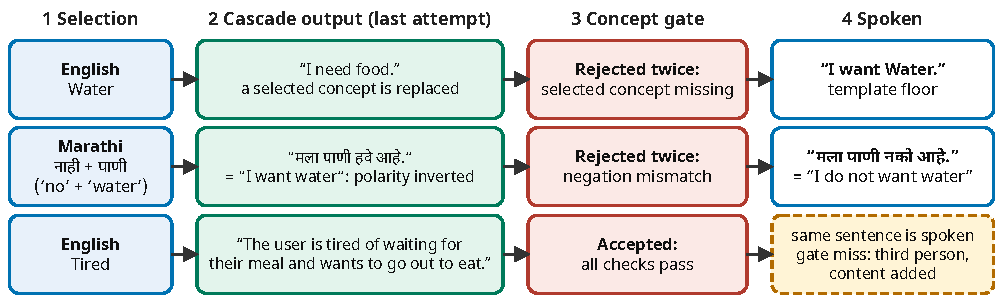
\includegraphics[width=\textwidth]{figures/teaser.pdf}
\caption{Three recorded requests from the frozen evaluation. The gate rejects a cascade output that replaces a selected concept (row~1) or inverts polarity (row~2, explicit negation field) and speaks a template built from the user's labels; it accepts a fluent third-person sentence that adds content (row~3, a miss). Marathi glosses are given in quotation marks.}
\label{fig:teaser}
\end{figure*}


\begin{abstract}
Symbol-based augmentative and alternative communication (AAC) devices voice telegraphic labels, whereas Hindi, Gujarati, and Marathi sentences need case marking, agreement, and negation.
A language model can expand a selection into a sentence, but it can also replace a concept, drop a negation, or add content, and an AAC device speaks for its user.
We present \sys{}, a web system for English, Hindi, Gujarati, and Marathi that speaks a model-generated sentence only if a deterministic gate confirms the selected concepts, polarity, and intended act, and otherwise speaks a template built from the user's own labels.
On \NPrimAll{} frozen scenarios sent as the web client builds them, the gate raises success from \XPreUSuccPct{} to \XDepUSuccPct{} and keeps all \NConc{} required concept instances (the ungated cascade keeps \XPreUKept{}) with no polarity error; with explicit intent fields, success rises from \XPreSSuccPct{} to \XDepSSuccPct{}.
A template alone reaches \XTmplUSuccPct{} and \XTmplSSuccPct{}, so under a lexical scorer the gate is a safeguard and not a quality gain.
The failure audit produced a repaired build, scored here only as a regression check.
A suffix-trie predictor exceeds trigram backoff by 1.1 hit@1 points in English and 1.2 in Hindi.
Speech synthesis is integrated but was not evaluated; a reviewer package and a screencast accompany the submission.
\end{abstract}

\section{Introduction}
\label{sec:intro}

A person who communicates through a symbol-based AAC board composes a message by tapping pictograms, and the device voices the selected labels.
The message is telegraphic (\emph{Water}, or \emph{No}\,+\,\emph{Pizza}) and the listener cannot see the selection, so a fluent sentence that misstates it can cause harm when the message is a request, a refusal, or a report of pain.
For a water request, a single \emph{Water} symbol can be realized as a complete sentence in each language, with a verb-final, experiencer-dative construction for the want:

\begin{center}
\small\renewcommand{\arraystretch}{1.12}
\begin{tabular}{@{}lll@{}}
\lang{Hindi} & \hi{मुझे पानी चाहिए।} & \multirow{3}{*}{\gloss{I want water.}}\\
\lang{Gujarati} & \gu{મને પાણી જોઈએ છે.} & \\
\lang{Marathi} & \hi{मला पाणी हवे आहे.} & \\
\end{tabular}
\end{center}

Feelings and negation use other constructions, so a literal join of labels is hard to parse.
A language model can generalize across combinations, but the small model that fits a 4\,GB GPU in our setup, \qwen{}, produced a successful sentence for only \XNaiveSucc{} of our scenarios when prompted without constraints (Section~\ref{sec:eval}).
Even when fluent, the cascade evaluated here fails in three ways (Figure~\ref{fig:teaser}): it replaced the concept for \emph{Water}, inverted polarity for Marathi \emph{No}\,+\,\emph{Water}, and added content for \emph{Tired}; with explicit negation, it dropped or inverted polarity in \XPreSPol{} scenarios.

\sys{} treats the selection as a contract.
A \emph{concept ledger} lists the concepts that must appear and those that must not; a prompted cascade proposes a sentence; a deterministic \emph{gate} accepts it only if its checks on concepts, polarity, and communicative act pass; and otherwise a template built from the user's own labels is spoken.
\qwen{} and \indicf{} are used as released.
Our contribution is the application and evaluation of explicit concept, polarity, and act checks in an Indic symbol-to-speech workflow, including the consequences of its fallback policy, for symbol-board users and the caregivers and clinicians who configure boards.

\begin{itemize}
\item \textbf{Concept-gated realization:} a ledger, a four-part acceptance rule, retry, and a template floor (Section~\ref{sec:system}).
\item \textbf{A four-language demo} with predictors trained on AAC dialogues (Section~\ref{sec:system}, Appendix Table~\ref{tab:models}).
\item \textbf{A frozen, paired evaluation} of \NPrimAll{} scenarios and the audit-driven repair (Sections~\ref{sec:eval} and~\ref{sec:repair}).
\end{itemize}

\section{Related Work}
\label{sec:related}

\paragraph{Expanding telegraphic input.}
Compansion expanded telegraphic AAC input into well-formed English sentences with syntactic and semantic rules \citep{mccoy1998compansion}.
Recent systems apply language models to other inputs. SpeakFaster expands abbreviated text for eye-gaze typists \citep{cai2024speakfaster}; ConnecTone suggests text from conversational context and speaks it with a style-adaptive TTS \citep{francis2024connectone}; \citet{mohan2024composition} compose messages from typed, emoji, or spoken input in the user's own voice.
\citet{karmakar-sinha-2024-aiding} contribute a symbol-to-text dataset, a text-to-pictogram module, and an extension to Bengali.
\sys{} starts from symbol selections, which give the model a small concept set whose omission or inversion can be checked; its novelty lies in that check and its evaluation, not in the expansion itself.

\paragraph{Boards and voices.}
Cboard is an open-source web board that states support for 46 languages without naming Hindi, Gujarati, or Marathi \citep{cboard}; Jellow lists 24 languages including all three, speaks pre-made sentences, and lets users type new ones \citep{jellow}; Avaz provides regional vocabularies and predictive text \citep{avaz}, and its FreeSpeech app teaches grammar by sentence building \citep{avazfreespeech}.
\citet{francis2025static} add generated symbols and zero-shot voice cloning to a symbol board.

\paragraph{Gap.}
Table~\ref{tab:related} compares documented capabilities (\nstated{}: not stated by the source, not absent).
Among these sources, none documents a deterministic check that preserves selected concepts and polarity in model-generated Indian-language sentences on a symbol board; we make no claim about undocumented products.

\begin{table*}[t]
\centering\footnotesize
\setlength{\tabcolsep}{3.6pt}\renewcommand{\arraystretch}{1.1}
\begin{tabular}{@{}L{2.75cm}L{2.2cm}L{2.75cm}L{2.7cm}L{2.15cm}L{1.95cm}@{}}
\toprule
\rowcolor{headtint}
System & Input & Languages (as stated) & Sentence realization & Output check & Speech \\
\midrule
Compansion & telegraphic words & English & rule-based expansion & \nstated & \nstated \\
\citeauthor{karmakar-sinha-2024-aiding} & symbols, text & incl.\ Bengali & symbol-to-text data & \nstated & \nstated \\
Cboard & symbols, text & 46; HI, GU, MR not named & \nstated & \nstated & text-to-speech \\
Jellow & symbols, keyboard & 24, incl.\ HI, GU, MR & pre-made, typed & \nstated & Google TTS \\
ConnecTone & speech, text & \nstated & context suggestions & \nstated & adaptive TTS \\
SpeakFaster & abbreviated text & \nstated & LLM expansion & \nstated & \nstated \\
\midrule
\rowcolor{rowtint}\textbf{\sys{}} & symbols, text & EN, HI, GU, MR & prompted \llm{Qwen} cascade & concept, polarity, act gate & \llm{IndicF5}, browser \\
\bottomrule
\end{tabular}
\caption{Documented capabilities of the closest systems, from the cited paper or the vendor page (read 2026-11-12; Jellow and \citeauthor{karmakar-sinha-2024-aiding} re-read 2026-11-13). \nstated{}: not stated by the source.}
\label{tab:related}
\end{table*}

\section{System Design and Demo Walkthrough}
\label{sec:system}

\begin{figure*}[t]
\centering
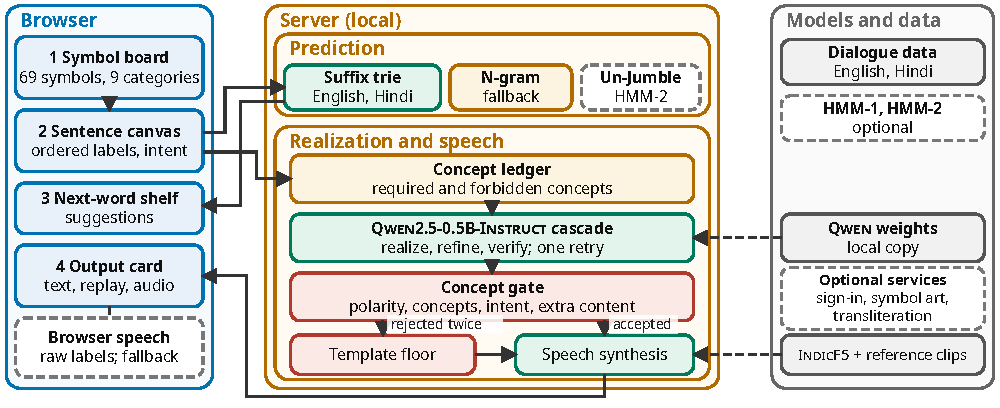
\includegraphics[width=0.92\textwidth]{figures/architecture.pdf}
\caption{Architecture of \sys{}. A selection in the browser goes to the server for next-word suggestions and for realization. The cascade output is spoken only if the gate accepts it; after two rejections a template built from the user's labels is spoken. Dashed boxes are optional components.}
\label{fig:arch}
\end{figure*}

\paragraph{Walkthrough.}
Figure~\ref{fig:arch} shows the decision path from a selection to the spoken sentence.
The user picks a language and taps symbols from a board of \NSymbols{} symbols in \NCategories{} categories, labeled in English, Hindi, Gujarati, and Marathi (Figure~\ref{fig:ui}, \cn{1}), or types free text.
Selections accumulate on a sentence canvas (\cn{2}), and a shelf proposes next words with their probabilities (\cn{3}).
\emph{Speak} voices the literal labels with the browser's speech synthesis; \emph{AI Polish \& Speak} (\cn{4}) sends the selection to the server, which returns a sentence that the output card shows while it is spoken (\cn{5}).
Quick Express speaks emergency phrases in one tap, Un-Jumble reorders canvas words with a second HMM, and an accessibility dock adjusts size, contrast, and speech speed.

\begin{figure}[t]
\centering
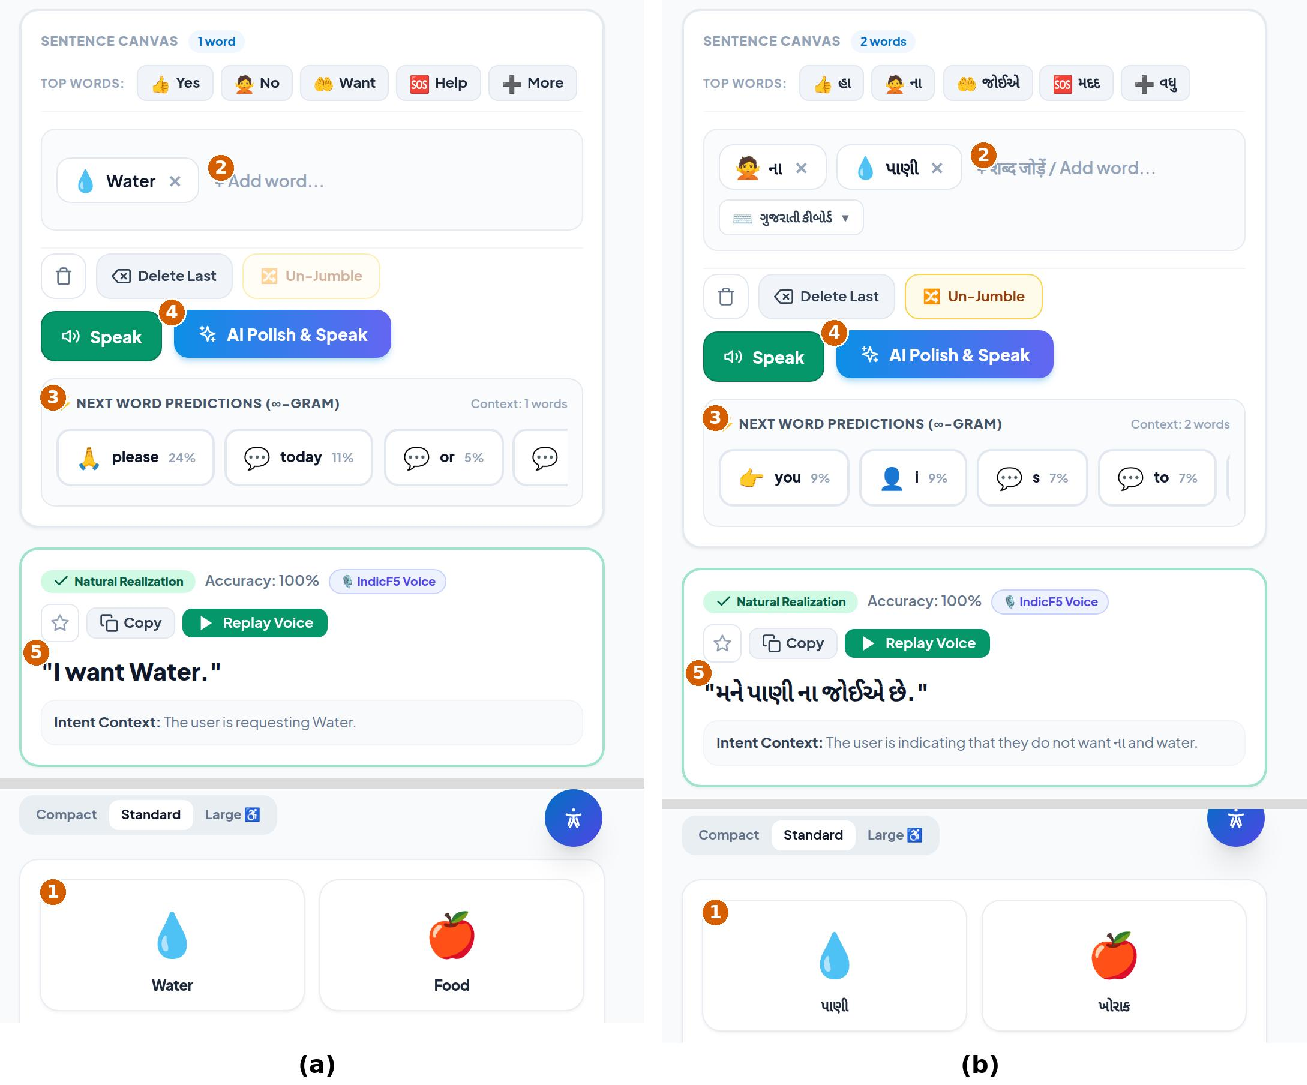
\includegraphics[width=0.9\columnwidth]{figures/ui_panel.pdf}
\caption{The running build (Chrome, 520\,px viewport). (a)~English \emph{Water}: the cascade output was rejected and the template was spoken. (b)~Gujarati \gu{ના}\,+\,\gu{પાણી} (\emph{no}\,+\,\emph{water}): the cascade output was accepted. Callouts: \cn{1} symbol, \cn{2} canvas, \cn{3} next-word shelf, \cn{4} generate, \cn{5} output. The \emph{Accuracy} badge is the validator's heuristic score, not a gate threshold.}
\label{fig:ui}
\end{figure}

\paragraph{Request and concept ledger.}
The browser sends the ordered labels with the communicative intent (request, statement, question, or negation), a negation indicator, the language, and an optional code-mixing indicator.
The evaluated client infers intent and negation from label substrings (a negator in a label means negation, question words a question, a few feeling labels a statement, anything else a request); any other client can supply both fields explicitly, the \emph{explicit} condition of Section~\ref{sec:eval}.
The server builds a \emph{ledger}: a required set (intent, speaker, each selected concept, negation) and a forbidden set of 21 default words for unrequested times, meals, and venues, minus any word the user selected.

\paragraph{Realization and gate.}
Three prompted stages share one frozen \qwen{} \citep{qwen2025qwen25}.
The realizer writes a sentence from a few-shot prompt for Hindi, Gujarati, and Marathi (12, 9, and 9 examples; greedy decoding) and from a ledger prompt for English and code-mixed output (temperature 0.1); the refiner removes unsupported content and is skipped for Indic-script candidates; the verifier returns a verdict and a minimal rewrite, which is advisory.
The gate decides by Equation~\eqref{eq:gate}, with $\nu$ the negation indicator, $E$ the selected concepts, $F$ the forbidden set, and $y$ the candidate:
\begin{equation}
\begin{split}
\mathrm{acc}(y)={}&[\mathrm{neg}(y)=\nu]\wedge\mathrm{match}(E,y)\wedge\mathrm{intent}(y)\\
&\wedge\neg\mathrm{forbid}(y)\wedge\neg\mathrm{time}(y).
\end{split}
\label{eq:gate}
\end{equation}
Here \emph{neg} tests lists of English, Hindi, Gujarati, and Marathi negators; \emph{match} requires every selected concept to appear (a substring, plural, and Indic-stem test); \emph{intent} rejects ``I want'' for feeling intents and requires a question cue for questions; \emph{forbid} matches a word of $F$; and \emph{time} flags time words when none was selected.
A rejection triggers one more cascade run, and after two rejections a language-specific template built from the selected labels (e.g., ``I want Water.'') is returned; English and code-mixed retries resample, whereas greedy Indic retries repeat.

\paragraph{Prediction, speech, and training.}
Next-word suggestions come from an unbounded-order suffix trie in the spirit of infini-gram \citep{liu2024infinigram}, built in under a second at start-up from the English and Hindi AAC dialogues (\IGSent{} sentences, maximum depth \IGDepth{}). Marathi reuses the Hindi trie and Gujarati has no predictor; two HMMs trained on streamed text (HMM-1 for next words, HMM-2 for Un-Jumble) are optional components that the evaluated build ran without.
The returned sentence is synthesized by \indicf{} \citep{ai4bharat2025indicf5}, a flow-matching model of the F5-TTS family \citep{chen2025f5tts}, with a 24\,kHz \vocos{} vocoder \citep{siuzdak2023vocos}, conditioned zero-shot on a reference clip and its transcript.
The model card lists Hindi, Gujarati, and Marathi but not English, so the English route is unverified; browser speech voices the literal labels and serves as the fallback (Appendix~\ref{app:coverage}).
In the evaluated build neither route produced speech: the gated \indicf{} weights were absent, so the server returned a placeholder tone, and headless Chrome exposed no voices.
\qwen{} is prompted and \indicf{} is used as released; we train the suffix trie, a Hindi HMM, two English HMMs, and an English \flant{} refiner (Appendix Table~\ref{tab:models}).

\section{Evaluation}
\label{sec:eval}

\paragraph{Protocol.}
We froze \NScen{} monolingual and \NScenCM{} exploratory Hinglish scenarios before scoring any output.
Each of English, Hindi, Gujarati, and Marathi has 46 board selections in six families (Appendix Table~\ref{tab:type}), with gold polarity and act fixed.
Each scenario is sent as the web client builds it (\emph{client}, the primary condition, because it is what a user's taps produce) and with explicit intent and negation fields (\emph{explicit}, a controlled diagnostic of the cost of inferring intent and not a measure of user-selected intent).

\paragraph{Systems and scoring.}
We compare (i) a literal join of the labels; (ii) the same \qwen{} with one unconstrained prompt; (iii) the cascade output before the gate, from the same response as the deployed output; (iv) the deployed output of the live server (one GTX~1650, 4\,GB); and (v) the template alone.
A scenario \emph{succeeds} if the output keeps every selected concept, has the gold polarity and act, adds no unselected concept, and is a first-person sentence in the target script; \emph{retention} counts the \NConc{} required concept instances separately.
A lexical scorer written independently of the gate applies these rules (Appendix~\ref{app:scorer}); all counts here use its first version, and Section~\ref{sec:repair} reports its correction.
Nine of the \NScen{} scenarios, whose few-shot prompt reproduces a prompt example, are excluded, leaving \NPrimAll{} (EN \NPrimEN{}, HI \NPrimHI{}, GU \NPrimGU{}, MR \NPrimMR{}).
Differences are paired, with 95\% bootstrap intervals over the 46 scenario groups (the four language versions of one board selection; 10,000 resamples).

\begin{table*}[t]
\centering\footnotesize
\setlength{\tabcolsep}{3.2pt}
\begin{tabular}{@{}l ccccc @{\hspace{6pt}} c ccccc@{}}
\toprule
 & \multicolumn{5}{c}{Scenario success (n/N)} & \multicolumn{6}{c}{Pooled diagnostics (counts)} \\
\cmidrule(lr){2-6}\cmidrule(l){7-12}
System & EN & HI & GU & MR & All & Kept$\uparrow$ & Pol.$\downarrow$ & \shortstack{Wrong\\act$\downarrow$} & \shortstack{No\\act$\downarrow$} & Added$\downarrow$ & \shortstack{Off-\\task$\downarrow$} \\
\midrule
\multicolumn{12}{@{}l}{\emph{Payload built by the web client (intent and negation inferred from labels)}}\\
Unconstrained Qwen & 2/46 & 1/45 & 4/42 & 1/42 & 8/175 & 199/215 & 2 & 3 & 163 & 7 & 16 \\
Cascade before gate & 3/46 & 24/45 & 20/42 & 18/42 & 65/175 & 175/215 & 2 & 54 & 33 & 25 & 19 \\
\rowcolor{rowtint}\textbf{\sys{} (deployed)} & \textbf{22/46} & \textbf{31/45} & \textbf{21/42} & \textbf{23/42} & \textbf{97/175} & \textbf{215/215} & \textbf{0} & \textbf{54} & \textbf{21} & \textbf{4} & \textbf{10} \\
Template floor & 33/46 & 31/45 & 27/42 & 27/42 & 118/175 & 215/215 & 0 & 57 & 0 & 0 & 0 \\
\midrule
\multicolumn{12}{@{}l}{\emph{Payload with explicit intent and negation fields}}\\
Cascade before gate & 5/46 & 26/45 & 16/42 & 24/42 & 71/175 & 185/215 & 36 & 30 & 44 & 21 & 17 \\
\rowcolor{rowtint}\textbf{\sys{} (deployed)} & \textbf{33/46} & \textbf{41/45} & \textbf{26/42} & \textbf{32/42} & \textbf{132/175} & \textbf{215/215} & \textbf{0} & \textbf{17} & \textbf{24} & \textbf{3} & \textbf{9} \\
Template floor & 46/46 & 45/45 & 34/42 & 42/42 & 167/175 & 215/215 & 0 & 0 & 8 & 0 & 0 \\
\bottomrule
\end{tabular}
\caption{Primary set (175 scenarios; EN 46, HI 45, GU 42, MR 42), scorer version 1. Success requires every selected concept, the gold polarity and act, no added concept, and an on-task first-person sentence in the target script. Kept: required concept instances present (of 215). Pol., Wrong act, No act, Added, Off-task: scenarios (of 175) with that error; one output can have several. Off-task: a model refusal or meta-comment, a third-person report, empty or over-long text, or Latin text in an Indic target (a user's own refusal never is). A literal join of the labels succeeds on 0/175 scenarios, as it carries no act marker by construction.}
\label{tab:results}
\end{table*}

\begin{table}[t]
\centering\footnotesize
\setlength{\tabcolsep}{3pt}
\begin{tabular}{@{}lcccccc@{}}
\toprule
 & \multicolumn{3}{c}{English} & \multicolumn{3}{c}{Hindi} \\
\cmidrule(lr){2-4}\cmidrule(l){5-7}
Model & @1 & @5 & MRR & @1 & @5 & MRR \\
\midrule
Unigram frequency & 3.6 & 11.6 & 0.069 & 6.4 & 14.5 & 0.099 \\
Bigram, backoff & 13.6 & 29.5 & 0.204 & 24.0 & 43.1 & 0.320 \\
Trigram, backoff & 16.0 & 32.8 & 0.234 & 25.9 & 44.0 & 0.334 \\
Gutenberg HMM & 6.7 & 15.5 & 0.105 & -- & -- & -- \\
Hindi AAC HMM & -- & -- & -- & 24.5 & 41.9 & 0.315 \\
\midrule
\rowcolor{rowtint}\textbf{$\infty$-gram (deployed)} & \textbf{17.2} & \textbf{33.4} & \textbf{0.240} & \textbf{27.0} & \textbf{44.1} & \textbf{0.343} \\
\bottomrule
\end{tabular}
\caption{Next-word prediction on AAC-user utterances: 60 of the 300 source conversations per language are held out (240 train), giving 2,220 English and 2,437 Hindi contexts; hit rates in \%, MRR@10. The n-gram baselines, the trie, and the Hindi HMM share the training split; the Gutenberg HMM is trained on public-domain books. Held-out sources share 18 of 392 English and 28 of 384 Hindi distinct utterances with training; \PredOOVEN{} (EN) and \PredOOVHI{} (HI) of targets are out of vocabulary and count as misses. Gujarati and Marathi are not evaluated because no AAC dialogue corpus exists for them.}
\label{tab:pred}
\end{table}


\paragraph{RQ1: the gate preserves what the cascade loses.}
Before the gate, the cascade keeps \XPreUKeptPct{} of required concepts under client payloads (\XPreSKeptPct{} with explicit fields) and, with explicit fields, makes \XPreSPol{} polarity errors, \XPolDropPreS{} of them dropped negations (Table~\ref{tab:results}).
With the gate and template floor, the same requests keep all \NConc{} concepts and make no polarity error on this benchmark; these counts describe what the implemented checks test, not a guarantee of meaning.
Success rises from \XPreUSucc{} to \XDepUSucc{} under client payloads (+18.3 percentage points, 95\% CI 11.9 to 25.2) and from \XPreSSucc{} to \XDepSSucc{} with explicit fields (+34.9, 26.7 to 43.4).
Gains concentrate in refusals (10/38 to 38/38 with explicit fields) and negated feelings (2/32 to 13/32; Appendix Table~\ref{tab:type}).
With explicit fields the gate lets model text through on \XGateAccPctS{} of requests (\XGateAccS{}/175); accepted outputs are fully correct in \XGateOkS{} and template fallbacks in \XFbOkS{} (Appendix~\ref{app:scorer} audits the failures); Appendix Figure~\ref{fig:workflow} follows one selection through all four languages.

\paragraph{RQ2: the remaining errors are mostly about intent.}
Under client payloads, \XDepUWrong{} deployed outputs express the wrong act; explicit fields cut this to \XDepSWrong{} and raise success from \XDepUSuccPct{} to \XDepSSuccPct{} (+20.0 points, 12.0 to 28.7).
The client infers \textsc{request} for \UIFeelReq{} of its 32 single-symbol feeling selections (8 feelings in 4 languages, counted before the nine exclusions; the primary set holds 30 feeling scenarios), so every language voices a feeling as a want (Table~\ref{tab:analysis}), and the gate's feeling test is an English pattern that does not catch it.
Two defects are independent of the model: the client's substring rule marks \UIFalseNeg{} of \UISingle{} single-symbol selections as negated (\emph{Nose} in English and Gujarati, \emph{Bathe} in Gujarati), and the template has no form for client intent \textsc{negation} (Table~\ref{tab:analysis}, second row).
Accepted outputs can also add content or a third-person perspective (Figure~\ref{fig:teaser}, row~3; Appendix Tables~\ref{tab:grid} and~\ref{tab:kinds}).

\begin{table*}[t]
\centering\footnotesize
\setlength{\tabcolsep}{3.4pt}\renewcommand{\arraystretch}{1.2}
\begin{tabular}{@{}L{2.35cm}L{2.95cm}L{3.0cm}L{3.1cm}L{3.1cm}@{}}
\toprule
\rowcolor{headtint}
Selection $\rightarrow$ intended & \lang{English} (baseline) & \lang{Hindi} & \lang{Gujarati} & \lang{Marathi} \\
\midrule
\emph{Angry} $\rightarrow$ \gloss{I am angry}
 & \bad{I want} \sel{Angry.} \routet\ \failmark{W}
 & \hi{\bad{मुझे} \sel{गुस्सा} \bad{चाहिए।}} \routem\ \failmark{W}
 & \gu{\bad{મને} \sel{ગુસ્સો} \bad{જોઈએ છે.}} \routem\ \failmark{W}
 & \hi{\bad{मला} \sel{रागात} \bad{हवे आहे.}} \routem\ \failmark{W} \\
\rowcolor{rowtint}
\emph{No}\,+\,\emph{Angry} $\rightarrow$ \gloss{I am not angry}
 & \bad{I want} \sel{No Angry.} \routet\ \failmark{W}
 & \hi{\sel{गुस्सा,} \bad{नहीं चाहिए।}} \routem\ \failmark{W}
 & \gu{\sel{મારે ના ગુસ્સો છે.}} \routem\ \failmark{N}
 & \hi{\bad{मला} \sel{नाही रागात} \bad{हवे आहे.}} \routet\ \failmark{W} \\
\bottomrule
\end{tabular}
\caption{One selection in four languages, deployed output with web-client input (recorded; glosses are the authors'). \sel{Blue}: selected concept kept; \kept{green}: successful sentence; \bad{red}: unwanted act or added content. \okmark{} success; \failmark{W} wrong act, \failmark{N} no act marker, \failmark{A} added content; \routem{} accepted model output, \routet{} template floor. English is the baseline language; the Indic columns are the proposed extension.}
\label{tab:analysis}
\end{table*}

\paragraph{RQ3: a template is a strong floor.}
A template echoes the selected labels, so it scores \XTmplSSucc{} with explicit fields and \XTmplUSucc{} under client payloads; the deployed pipeline trails it by 20.0 percentage points (95\% CI 14.0 to 26.4) and 12.0 (6.4 to 17.9), and ties it only in Hindi under client payloads.
Joining the eight explicit-field template failures by scenario identifier places all of them in Gujarati negated feelings. The valid template sentence \gu{મને ખુશ લાગતું નથી.} was missing from the scorer's marker list, whereas its Hindi and Marathi counterparts (\hi{मुझे खुश महसूस नहीं हो रहा है।} and \hi{मला आनंदी वाटत नाही.}) were recognized (all three: \gloss{I do not feel happy}); these are scorer gaps, not template errors.
The model path adds wrong-act outputs that a template does not (\XDepSWrong{} against \XTmplSWrong{}), and the lexical criterion rewards label echo without scoring fluency, so the comparison bounds what model phrasing adds without measuring it.

\paragraph{RQ4: next-word prediction.}
The suffix trie exceeds unigram and bigram baselines in both languages and a backoff trigram by \PredDENOneTri{} hit@1 in English (381 against 356 of 2,220 contexts) and \PredDHIOneTri{} in Hindi (659 against 630 of 2,437), computed from counts with a paired bootstrap over source conversations (Table~\ref{tab:pred}).

\section{From Audit to a Workable Build}
\label{sec:repair}

The audit traced the errors above to four defects, each repaired before any new scenario was drawn and frozen by recorded file hashes.
\textbf{Interface:} board symbols carry concept identifiers, intent is split into an act and a polarity field, typed words match only as whole tokens, and a message-type control and a two-button clarification card replace guessing; driving the real page, the original client sent a wrong act for 59 of 184 selections and the repaired client for none.
\textbf{Gate and templates:} the gate tests the writing system, speaker perspective, concept presence by identifier with inflected forms, added content, negation within the clause of the selected concept, and the act marker, with a reason code per rejection; compositional, locale-specific frames cover requests, refusals, feelings, negated feelings, actions, and calls for help, and an uncovered selection yields a labeled literal preview.
\textbf{Scorer:} version 2 adds the valid constructions that version 1 missed, moving the archived deployed count from 97 to 95 (client) and from 132 to 138 (explicit) and the template floor from 167 to 175.

\paragraph{Regression result.}
On the original \NPrimAll{} scenarios under version 2, the repaired hybrid and the repaired template both score 175/175 with client and explicit inputs (archived system: 95 and 138; matched one-pass \qwen{} prompt: 8/175), and the hybrid exceeds the same cascade without gate and fallback by 49.7 percentage points (95\% CI 42.3--57.1).
These scenarios informed the repairs, so 175/175 is a regression target and not a test result, and a lexical scorer cannot separate hybrid from template.
A fresh set of 120 scenarios (30 per language) was generated after the freeze; its gold annotation awaits two native speakers per language, so no score on it is reported, and blind native ratings of meaning and phrasing remain the pending test.

\section{Availability, License, and Limitations}
\label{sec:limits}

\paragraph{Availability and license.}
The reviewer package (source, frozen scenarios, scorer, raw outputs, installation guide) and a two-minute captioned screencast without audio are at \demourl{}.
Code is released under the \codelicense{}; the models and fonts keep their own licenses (Appendix Table~\ref{tab:models}), and installation tests are in Appendix~\ref{app:coverage}.

\paragraph{Limitations.}
The scorer is lexical and its Indic lexicon is not native-reviewed; scenarios cover one- and two-concept selections from a \NSymbols{}-symbol board; one team wrote the rules, gold annotation, and scorer without an independent curator; the Hindi dialogues are machine translations; English results are single samples; and no user study has been run, so the results bound lexical faithfulness and not communication effectiveness.
Speech was synthesized in placeholder mode, so latency (Appendix~\ref{app:coverage}) excludes synthesis and speech quality was not assessed.
Gujarati has no predictor and Marathi reuses the Hindi trie, so extending Table~\ref{tab:pred} to both is the next phase and needs AAC dialogue corpora for them.
In the evaluated build the fallback template is not re-validated and the gate's intent test covers English cues only.

\section{Conclusion}
\label{sec:conclusion}

A small prompted language model can sit in front of an AAC voice when a deterministic gate decides what is spoken.
Across \NPrimAll{} frozen scenarios in four languages, the gate kept every selected concept and removed all polarity errors, while the template floor, which speaks only the user's own labels, matched or exceeded the pipeline under a lexical scorer.
The audit produced a repaired build that now serves as a regression target; native-speaker confirmation of a fresh scenario set, blind ratings of meaning and phrasing, and real speech in all four languages are the next steps toward measuring what model phrasing adds.


\section*{Ethics Statement}
An AAC device speaks for a person, so a plausible but wrong sentence can misstate consent or refusal.
The gate lowers this risk without removing it: it checks selected concepts, polarity, and a limited set of intent cues, not meaning in full.
The evaluated interface speaks a sentence as soon as it is ready and does not show when a template replaced model output; the repaired build labels templates and does not speak a clarification or a literal preview unprompted, but consequential messages should still be confirmed with the user or a caregiver, and a preview-and-confirm step for generated sentences is a priority for deployments.
Direct \emph{Speak} and Quick Express remain available when generated text is unsuitable.

Voice cloning requires a reference clip and its exact transcript from the speaker or a guardian, with consent; clones are held in server memory only.
Optional features can send typed words to third parties (Google Input Tools, OpenAI Images) or store My Words and bookmarks in Firebase; generation, prediction, and speech do not need them.
The evaluation uses synthetic dialogues and scripted scenarios and contains no personal data; a study with AAC users would need accessible consent and the option to withdraw data.
Accessibility testing covered keyboard activation, emulated touch, and automated checks of names and live regions, not screen readers or switch scanning; the page has no live region for new text and renders nothing when the content delivery networks that serve its React, Babel, and Tailwind libraries are blocked, although generation and prediction run on the local server.
The evaluated build ran without the HMM-1 and HMM-2 checkpoints, so HMM-1 prediction and Un-Jumble are not evaluated.


\section*{Acknowledgements}
We used generative AI assistants (Claude by Anthropic; ChatGPT and Codex by OpenAI) to merge two snapshots of the system into the version evaluated here, write the evaluation harness and scorer, repair the interface, gate, and templates described in Section~\ref{sec:repair}, and draft and edit this paper.
All reported numbers are regenerated from the recorded result files.
The AAC dialogue data were generated with OpenAI gpt-4o-mini, and the Hindi dialogues are machine translations (opus-mt-en-hi).


\bibliography{references}

\clearpage
\appendix
\twocolumn[{%
\makeatletter
\section{Interaction Trace and Test Cases}\label{app:trace}\label{app:tests}
\centering
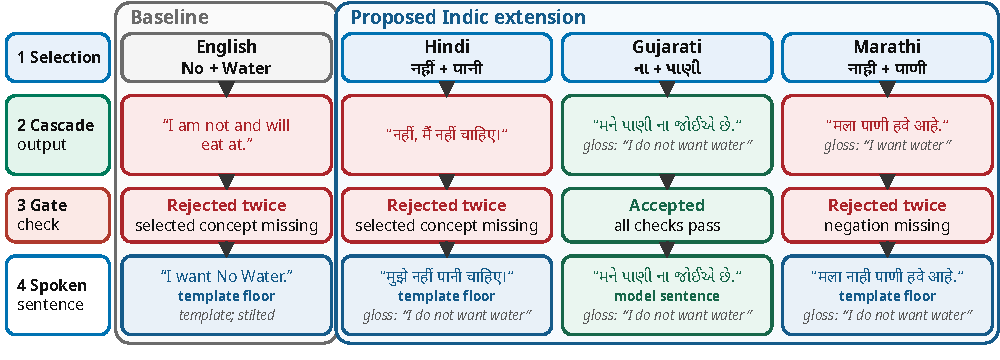
\includegraphics[width=\textwidth]{figures/fig4_languages.pdf}
\captionof{figure}{One selection (\emph{No}\,+\,\emph{Water}) in four languages (recorded outputs). English is the baseline language; Hindi, Gujarati, and Marathi are the proposed extension. Red: rejected cascade output; blue: template floor; green: accepted model sentence; italics: the authors' English gloss. The word order of the template sentences is not native-reviewed.}
\label{fig:workflow}
\vspace{2pt}
\centering\footnotesize
\setlength{\tabcolsep}{3.2pt}\renewcommand{\arraystretch}{1.1}
\begin{tabular}{@{}L{2.5cm}L{2.95cm}L{2.85cm}L{3.0cm}L{3.0cm}@{}}
\toprule
\rowcolor{headtint}
Family: selection & \lang{English} (baseline) & \lang{Hindi} & \lang{Gujarati} & \lang{Marathi} \\
\midrule
Request: \emph{Fruit}
 & \kept{I want Fruit.} \routet\ \okmark
 & \hi{\kept{मुझे फल चाहिए।}} \routem\ \okmark
 & \gu{\kept{મને ફળ જોઈએ છે.}} \routem\ \okmark
 & \hi{\kept{मला फळ हवे आहे.}} \routem\ \okmark \\
\rowcolor{rowtint}
Refusal: \emph{No}\,+\,\emph{Fruit}
 & \bad{I am not a} \sel{fruit}\bad{. I do not eat fruits.} \routem\ \failmark{W,A}
 & \hi{\kept{फल नहीं है, नहीं चाहिए।}} \routem\ \okmark
 & \gu{\sel{મારે ના ફળ છે.}} \routem\ \failmark{N}
 & \hi{\kept{मला नाही फळ हवे आहे.}} \routet\ \okmark \\
Feeling: \emph{Angry}
 & \bad{I want} \sel{Angry.} \routet\ \failmark{W}
 & \hi{\bad{मुझे} \sel{गुस्सा} \bad{चाहिए।}} \routem\ \failmark{W}
 & \gu{\bad{મને} \sel{ગુસ્સો} \bad{જોઈએ છે.}} \routem\ \failmark{W}
 & \hi{\bad{मला} \sel{रागात} \bad{हवे आहे.}} \routem\ \failmark{W} \\
\rowcolor{rowtint}
Negated feeling: \emph{No}\,+\,\emph{Angry}
 & \bad{I want} \sel{No Angry.} \routet\ \failmark{W}
 & \hi{\sel{गुस्सा,} \bad{नहीं चाहिए।}} \routem\ \failmark{W}
 & \gu{\sel{મારે ના ગુસ્સો છે.}} \routem\ \failmark{N}
 & \hi{\bad{मला} \sel{नाही रागात} \bad{हवे आहे.}} \routet\ \failmark{W} \\
Action: \emph{Drink}\,+\,\emph{Milk}
 & \bad{The user requested} \sel{milk} \bad{for their drink.} \routem\ \failmark{N,P}
 & \hi{\kept{मुझे पीना दूध चाहिए।}} \routet\ \okmark
 & \gu{\kept{મને પીવું જોઈએ છે. દૂધ આપે.}} \routem\ \okmark
 & \hi{\kept{मला पिणे दूध हवे आहे.}} \routem\ \okmark \\
\rowcolor{rowtint}
Call: \emph{Call}\,+\,\emph{Doctor}
 & \kept{I want Call Doctor.} \routet\ \okmark
 & \hi{\kept{फ़ोन करना गया है, मुझे डॉक्टर चाहिए।}} \routem\ \okmark
 & \gu{\sel{મને ડૉક્ટર ફોન કરવો છે.}} \routem\ \failmark{N}
 & \hi{\sel{मला डॉक्टर फोन करणे मिळू शकता का?}} \routem\ \failmark{N} \\
\bottomrule
\end{tabular}
\captionof{table}{One scenario per family (the first in alphabetical order that is in the primary set for all four languages), deployed output with web-client input (recorded). Intended messages: \gloss{I want fruit}, \gloss{I do not want fruit}, \gloss{I am angry}, \gloss{I am not angry}, \gloss{I want to drink milk}, \gloss{I want to call the doctor}. Colors, marks, and tags as in Table~\ref{tab:analysis}; \failmark{P} is a third-person report. No native speaker has judged these outcomes; the Gujarati and Marathi \emph{Call} outputs are a scorer gap and a question form.}
\label{tab:grid}
\makeatother
}]

\begin{table*}[t]
\centering\footnotesize
\setlength{\tabcolsep}{3.2pt}\renewcommand{\arraystretch}{1.1}
\begin{tabular}{@{}L{2.6cm}L{3.0cm}L{6.2cm}L{3.2cm}@{}}
\toprule
\rowcolor{headtint}
Kind of outcome & Input & Recorded output & Result \\
\midrule
Concept replaced, caught & \lang{English}, client: \emph{Water} & cascade \bad{I need food.}; spoken \sel{I want Water.} \routet & rejected twice (selected concept missing) \\
\rowcolor{rowtint}Polarity inverted, caught & \lang{Marathi}, explicit: \emph{No}\,+\,\emph{Water} & cascade \hi{\bad{मला पाणी हवे आहे.}} (\gloss{I want water}); spoken \hi{\sel{मला पाणी नको आहे.}} \routet & rejected (negation missing); template \\
Accepted, third person & \lang{English}, client: \emph{Tired} & \bad{The user is tired of waiting for their meal and wants to go out to eat.} \routem & accepted by the gate; fails scorer (added content, third person) \\
\rowcolor{rowtint}Ambiguous selection; server unreachable (repaired client) & \lang{English}: \emph{Nose}; any language & card \gloss{What do you want to say?} with buttons \gloss{I want something} and \gloss{I feel something}; the literal labels, marked as a preview & nothing is spoken until the user chooses; nothing is guessed \\
\bottomrule
\end{tabular}
\caption{One recorded example of each further kind of outcome (colors and tags as in Table~\ref{tab:analysis}); the Gujarati scorer gap is in Section~\ref{sec:eval}. The last row shows demo states captured from the repaired build, not scored scenarios.}
\label{tab:kinds}
\end{table*}


\begin{table*}[t]
\centering\footnotesize
\setlength{\tabcolsep}{3pt}\renewcommand{\arraystretch}{1.08}
\begin{tabular}{@{}L{2.9cm}L{2.4cm}L{7.6cm}L{2.5cm}@{}}
\toprule
\rowcolor{headtint}
Component & Role in the demo & Training or adaptation & Data \\
\midrule
\qwen{} (rev.\ 7ae5576) & realizer, refiner, verifier & Prompted, not fine-tuned (few-shot for HI, GU, MR) & -- \\
\indicf{} + \vocos{} & speech & Pretrained; zero-shot voice conditioning on a clip and its transcript & 1,417\,h, four corpora \\
HMM-1, HMM-2 & optional next word; Un-Jumble & Streamed in 500K-sentence chunks, count-pruned; HMM-1: Jelinek--Mercer weights .50/.30/.15/.05; HMM-2: word and POS trigrams, beam 64 & English sentences, Tatoeba, Pile slices \\
Gutenberg HMM; Hindi AAC HMM & English baseline; Hindi fallback & Bigram and trigram counts over 188,402 sentences (713,845 trigram states); 3,867 Hindi turns, 2,171 word types (3,078 turns for evaluation) & public-domain books; Hindi dialogues \\
Suffix trie ($\infty$-gram) & primary next word & Count-based, built at start-up (\IGSent{} sentences, depth \IGDepth{}) & EN and HI dialogues \\
\flant{} refiner & companion tool & Fine-tuned: learning rate $10^{-4}$, batch 16 with two accumulation steps, 10 epochs, seed 42, one TITAN Xp (204\,s); 500-update fluency adaptation on 4,380 denoising pairs & 3,052 template payloads (384 validation, 384 test) \\
\bottomrule
\end{tabular}
\caption{Learned components, from the training records, run configurations, and model files in the release package; \qwen{} and \indicf{} are used as released. The \indicf{} corpora are Rasa, IndicTTS, LIMMITS, and IndicVoices-R. Licenses: \qwen{} Apache-2.0, \vocos{} MIT, \indicf{} MIT (gated download), Noto fonts SIL OFL 1.1. On its 384 test payloads the refiner reaches \RefAModel{} exact match (\RefFModel{} with the adaptation) and no negation error in 172 negated payloads, at a median of \RefALat{}\,ms; rules and the hybrid score \RefARules{} because the references come from the same template families.}
\label{tab:models}
\end{table*}

\section{Scorer Definitions and Failure Audit}
\label{app:scorer}
Retention is the share of required concept instances present (lexicon forms with inflection stems). Polarity is correct when a negator is present exactly if the gold message is negated, and the act is correct when a request marker (want, need, \hi{चाहिए}, \gu{જોઈએ}, \hi{हवे}) or, for feelings, a feeling marker without a request marker is present. A concept is \emph{added} if any other board concept or a time, meal, or venue word occurs.
An output is \emph{off-task} if it is a model refusal or meta-comment, a third-person report (``the user\ldots''), empty, longer than 25 tokens, or contains Latin text in an Indic target; a user's own refusal (\gloss{I do not want water}) is never off-task.
\emph{Failure audit.} Of the 37 accepted outputs that fail the scorer with explicit fields, 35 are genuine failures (12 negated want for a negated feeling, 10 ungrammatical, 9 third-person reports, 4 added content) and two are marker-list gaps, as are all six failing template fallbacks and all eight failing template-only outputs (the authors' classification, not native-checked).

\begin{table}[t]
\centering\footnotesize
\setlength{\tabcolsep}{2.6pt}
\begin{tabular}{@{}lcccccc@{}}
\toprule
 & \multicolumn{3}{c}{Client payload} & \multicolumn{3}{c}{Explicit fields} \\
\cmidrule(lr){2-4}\cmidrule(l){5-7}
Scenario family ($n$) & Pre & Dep. & Tmpl & Pre & Dep. & Tmpl \\
\midrule
Food/drink request (35) & 26 & 29 & 35 & 26 & 29 & 35 \\
Refusal (\emph{No}+food) (38) & 19 & 33 & 38 & 10 & 38 & 38 \\
Feeling (30) & 3 & 4 & 5 & 18 & 22 & 30 \\
Negated feeling (32) & 2 & 1 & 0 & 2 & 13 & 24 \\
Action + object (24) & 8 & 18 & 24 & 8 & 18 & 24 \\
Help/call + person (16) & 7 & 12 & 16 & 7 & 12 & 16 \\
\midrule
All (175) & 65 & 97 & 118 & 71 & 132 & 167 \\
\bottomrule
\end{tabular}
\caption{Successful scenarios by family on the primary set. Pre: cascade before the gate; Dep.: deployed output; Tmpl: template floor. Exploratory Hinglish ($n=8$; client, explicit): deployed \CMSuccDepU{}, \CMSuccDepS{}; unconstrained prompt \CMSuccNaive{}; template \CMSuccTmplU{}, \CMSuccTmplS{}.}
\label{tab:type}
\end{table}


\section{Language Coverage and Runtime}
\label{app:coverage}
Text generation and next-word coverage are described in Section~\ref{sec:system}. Speech goes to \indicf{} (English is not on its model card), with browser fallback voices hi-IN, gu-IN, and mr-IN (Gujarati and Marathi fall back to hi-IN, then en-IN) and en-US, en-IN, or en-GB; it was not verified in any language because the gated weights were absent and the test browser exposed no voices.
Gate-accepted requests took a median of \LatMedAccEN{}, \LatMedAccHI{}, \LatMedAccGU{}, and \LatMedAccMR{}\,s (EN, HI, GU, MR) and twice-rejected ones \LatFbMin{}--\LatFbMax{}\,s on the GTX~1650 (text generation only); on the repaired build, click to first playback of the placeholder tone had a median of 9.9\,s (95th percentile 20.8\,s; 31 warm runs), so time to audible speech is unmeasured.
In a fresh CPU environment the documented request took 44\,s (the weight download and a GPU installation were not tested); with downloads disabled and non-local connections refused, generation and prediction completed, the only outbound attempt being an optional service.



\end{document}
